\documentclass[a4paper, 12pt]{article}
\usepackage[T2A]{fontenc}
\usepackage[utf8]{inputenc}
\usepackage[english,russian]{babel}
\usepackage{amsmath, amsfonts, amssymb, amsthm, mathtools, misccorr, indentfirst, multirow}
\usepackage{wrapfig}
\usepackage{graphicx}
\usepackage{subfig}
\usepackage{enumitem}
\usepackage{adjustbox}
\usepackage{pgfplots}
\usepackage{caption}

\usepackage{geometry}
\geometry{top=20mm}
\geometry{bottom=20mm}
\geometry{left=20mm}
\geometry{right=20mm}
\newcommand{\angstrom}{\textup{\AA}}
\begin{document}
	\begin{titlepage}
		\begin{center}
		МИНИСТЕРСТВО ОБРАЗОВАНИЯ И НАУКИ РОССИЙСКОЙ ФЕДЕРАЦИИ\\
		\footnotesize{Московский физико-технический институт}\\
		\footnotesize{(государственный университет)}\\
		\vfill
		{\LARGE
		\textbf{Использование YAG:Nd$^{3+} $-лазера для гравировки материалов}\\
		}
		\vspace{1cm}
		Лабораторная работа по курсу\\
		фотоника
		\vfill
		\begin{flushright}
			Выполнили: студенты 654 и 653 групп.\\
			Нехаев А.С.\\
			Суманова Е.Д.\\
			Тихонов С.С.\\
			Хисматулина Е.А.\\
			Карпова Т.К.
		\end{flushright}
		\vfill
		г. Долгопрудный\\
		\the\year\:год
		\end{center}
	\end{titlepage}
	\newpage
	\pagenumbering{arabic}
	\tableofcontents
	\newpage
	\section{Цели и задачи исследования}
	\begin{enumerate}
		\item Изучить физические основы работы лазера в непрерывном режиме и режиме модуляции добротности;
		\item Исследовать зависимость мощности излучения от мощности накачки в режимах свободной генерации и модуляции добротности, т.е. найти КПД лазера в разных режимах работы;
		\item Исследовать зависимость ширины импульса от мощности накачки;
		\item Выгравировать изображение на пластиковой поверхности.	
	\end{enumerate}
	\newpage
	\section{Схема установки}
	\begin{figure}[h!]
	\begin{center}
		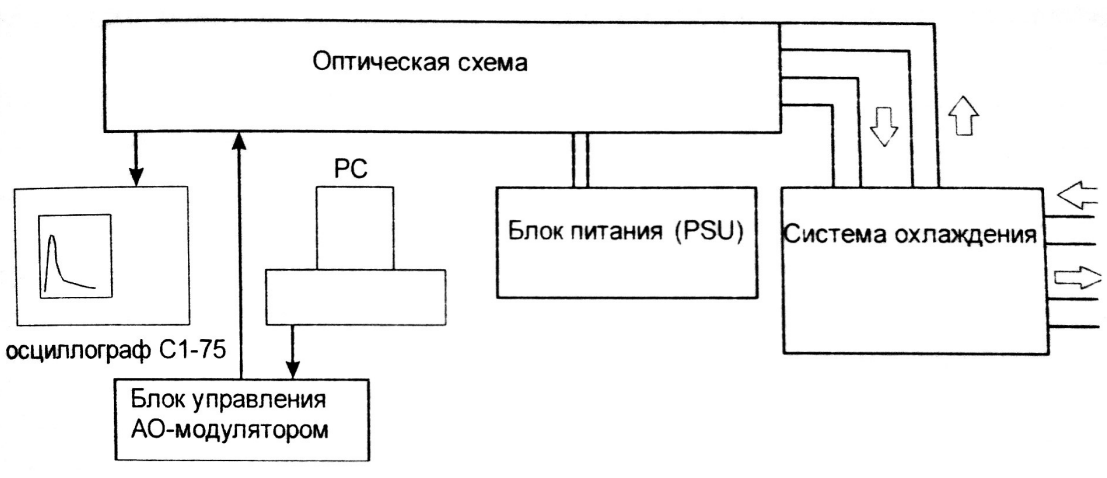
\includegraphics[scale = 0.4]{sch1}
		\caption{Принципиальная схема установки}
		\label{ris:shem1}
	\end{center}	
	\end{figure}
	\begin{figure}[h!]
	\begin{center}
		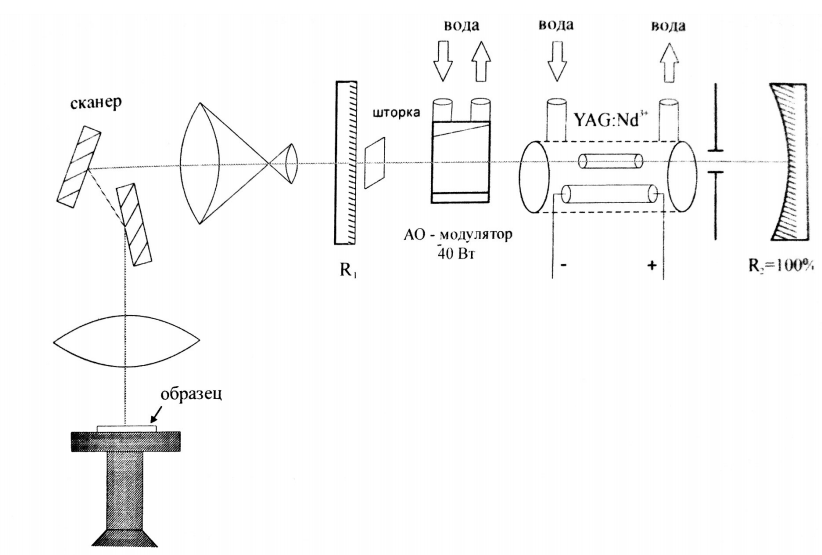
\includegraphics[scale = 0.44]{sch2}
		\caption{Схема оптической части}
		\label{ris:shem2}
	\end{center}	
	\end{figure}
	\section{Теоретичесое введение}
	
	В основе гравировки лазером лежит его тепловое воздействие на материал. При этом может происходить нагревание, плавление и испарение материала. Распределение тепла по материалу описывается уравнением теплопроводности, соответственно, к веществам с малым коэффициентом теплопроводности (например, металлам) необходимо применять короткоимпульсные лазеры, чтобы не взаимодействовать только с той областью материала, на которую попадает излучение. Отверстие наилучшей формы образуется в случае, если фокус лазера находится на поверхности материала. В этом случае определяющим процессом является испарение (рост отверстия вглубь), а ролью плавления (роста отверстия в ширину) можно пренебречь.\par
Описывать работу лазера принято \textit{скоростными уравнениями}:

\begin{equation}
\dfrac{dN}{dt} = R_p - B\phi N - \dfrac{N}{\tau},\quad
\dfrac{d\phi}{dt} = \left[BV_aN - \dfrac{1}{\tau_c}\right]\phi.
\label{eq_speed2}
\end{equation}
\par
Первое уравнение описывает изменение инверсии населённости, которое происходит из-за накачки, вынужденного и спонтанного излучений соответственно. Второе уравнение описывает изменение числа фотонов в резонаторе, обусловленное спонтанным излучением и временем жизни фотона в резонаторе.\par
В случае режима свободной генерации оба этих параметра принимают стационарные значения.
При модуляции добротности в лазере используется акустооптический модулятор, препятствующий генерации излучения путём увеличения потерь. Закрытый модулятор позволяет увеличивать рост инверсии заселённостей, а после открытия модулятора происходит генерация и резкое увеличесние числа фотонов в резонаторе. Таким образом, лазер может генерировать излучение в виде импульсов с большой пиковой мощностью, а из-за малой длительности импульса можно получить большую плотность мощности, что используется в обработке тугоплавких материалов.
\section{Результаты эксперимента}
\begin{table}[!htb]
	\centering
	\caption{Результаты измерений для режима свободной генерации.}
	\begin{tabular}{|c|c|c|c|}
	\hline
	Ток, А & Напряжение, В & Мощность накачки, мВт & Входная мощность, Вт\\
	\hline
 14.6 & 167. & 2. & 2438.2\\
 14.7 & 167. & 11. & 2454.9\\
 14.8 & 167. & 23. & 2471.6\\
 14.9 & 168. & 38. & 2503.2\\
 15. & 168. & 54. & 2520.\\
 15.1 & 168. & 72. & 2536.8\\
 15.2 & 169. & 95. & 2568.8\\
 15.3 & 169. & 116. & 2585.7\\
 15.4 & 169. & 131. & 2602.6\\
 15.5 & 170. & 152. & 2635.\\
 15.6 & 170. & 170. & 2652.\\
 15.7 & 170. & 194. & 2669.\\
 15.8 & 171. & 218. & 2701.8\\
 15.9 & 171. & 254. & 2718.9\\
 16. & 171. & 284. & 2736.\\
 16.1 & 172. & 320. & 2769.2\\
 16.2 & 172. & 354. & 2786.4\\
 16.3 & 172. & 386. & 2803.6\\
 16.4 & 173. & 425. & 2837.2\\
 16.5 & 173. & 464. & 2854.5\\
 16.6 & 173. & 490. & 2871.8\\
 16.7 & 174. & 538. & 2905.8\\
 16.8 & 174. & 599. & 2923.2\\
 16.9 & 175. & 642. & 2957.5\\
 17. & 175. & 690. & 2975.\\
 17.1 & 176. & 736. & 3009.6\\
 17.2 & 176. & 790. & 3027.2\\
 17.3 & 176. & 835. & 3044.8\\
 17.4 & 177. & 884. & 3079.8\\
 \hline
	\end{tabular}
\end{table}
\begin{table}[!htb]
	\centering
	\caption{Результаты измерений для режима модуляции добротности.}
	\begin{tabular}{|c|c|c|c|}
	\hline
	Ток, А & Напряжение, В & Мощность накачки, мВт & Входная мощность, Вт\\
	\hline
 14.4 & 167. & 2. & 2404.8 \\
 14.5 & 167. & 14. & 2421.5 \\
 14.6 & 168. & 35. & 2452.8 \\
 14.7 & 168. & 51. & 2469.6 \\
 14.8 & 168. & 69. & 2486.4 \\
 14.9 & 169. & 85. & 2518.1 \\
 15. & 169. & 102. & 2535. \\
 15.1 & 169. & 121. & 2551.9 \\
 15.2 & 170. & 140. & 2584. \\
 15.3 & 170. & 161. & 2601. \\
 15.4 & 170. & 182. & 2618. \\
 15.5 & 171. & 203. & 2650.5 \\
 15.6 & 171. & 232. & 2667.6 \\
 15.7 & 171. & 257. & 2684.7 \\
 15.8 & 172. & 284. & 2717.6 \\
 15.9 & 172. & 297. & 2734.8 \\
 16. & 172. & 325. & 2752. \\
 16.1 & 172. & 357. & 2769.2 \\
 16.2 & 173. & 397. & 2802.6 \\
 16.3 & 173. & 432. & 2819.9 \\
 16.4 & 174. & 470. & 2853.6 \\
 16.5 & 174. & 511. & 2871. \\
 16.6 & 174. & 531. & 2888.4 \\
 16.7 & 174. & 562. & 2905.8 \\
 16.8 & 175. & 602. & 2940. \\
 16.9 & 175. & 641. & 2957.5 \\
 17. & 175. & 686. & 2975. \\
 17.1 & 176. & 727. & 3009.6 \\
 17.2 & 176. & 772. & 3027.2 \\
 17.3 & 176. & 810. & 3044.8 \\
 17.4 & 177. & 854. & 3079.8 \\
 \hline
	\end{tabular}
\end{table}
\begin{figure}[!h]
	\minipage{0.48\textwidth}
	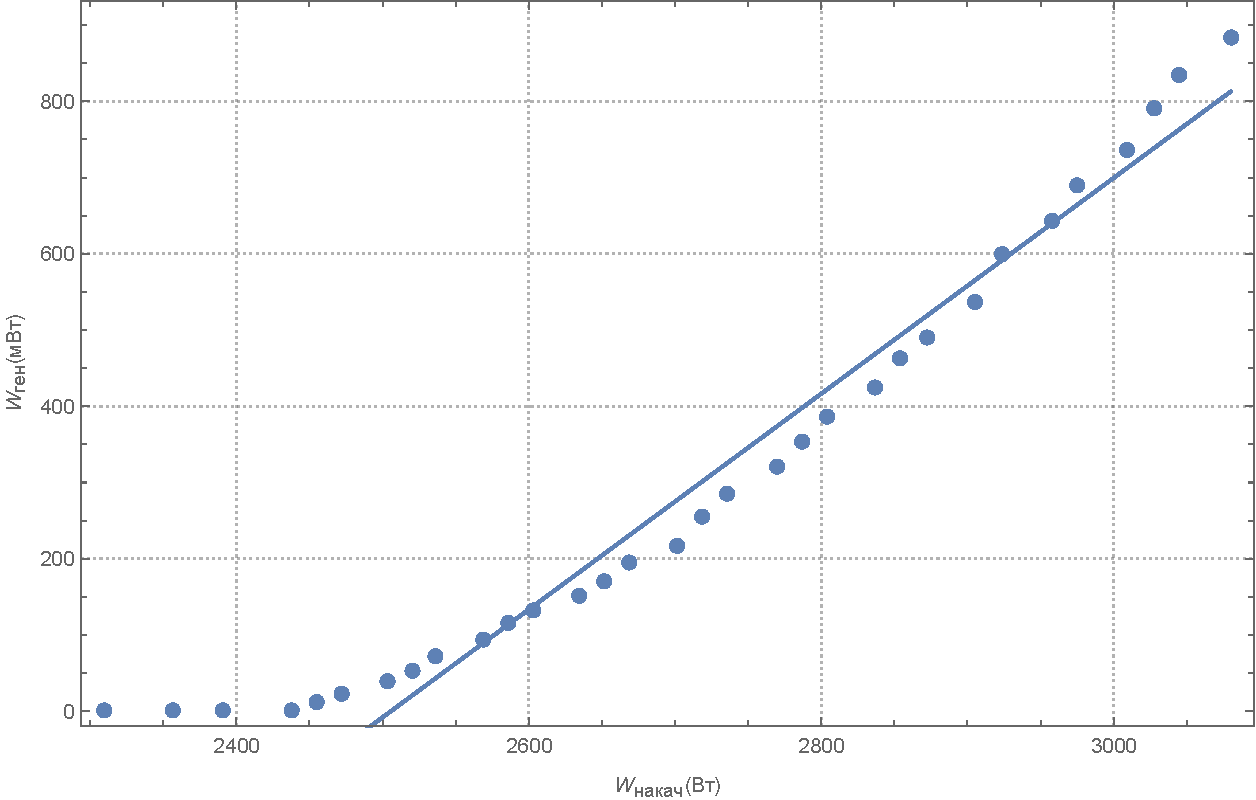
\includegraphics[width=\textwidth]{1.pdf}
	\caption{Зависимость мощности излучения от мощности накачки в режиме свободной генерации}
	\endminipage
	\hfill
	\minipage{0.48\textwidth}
	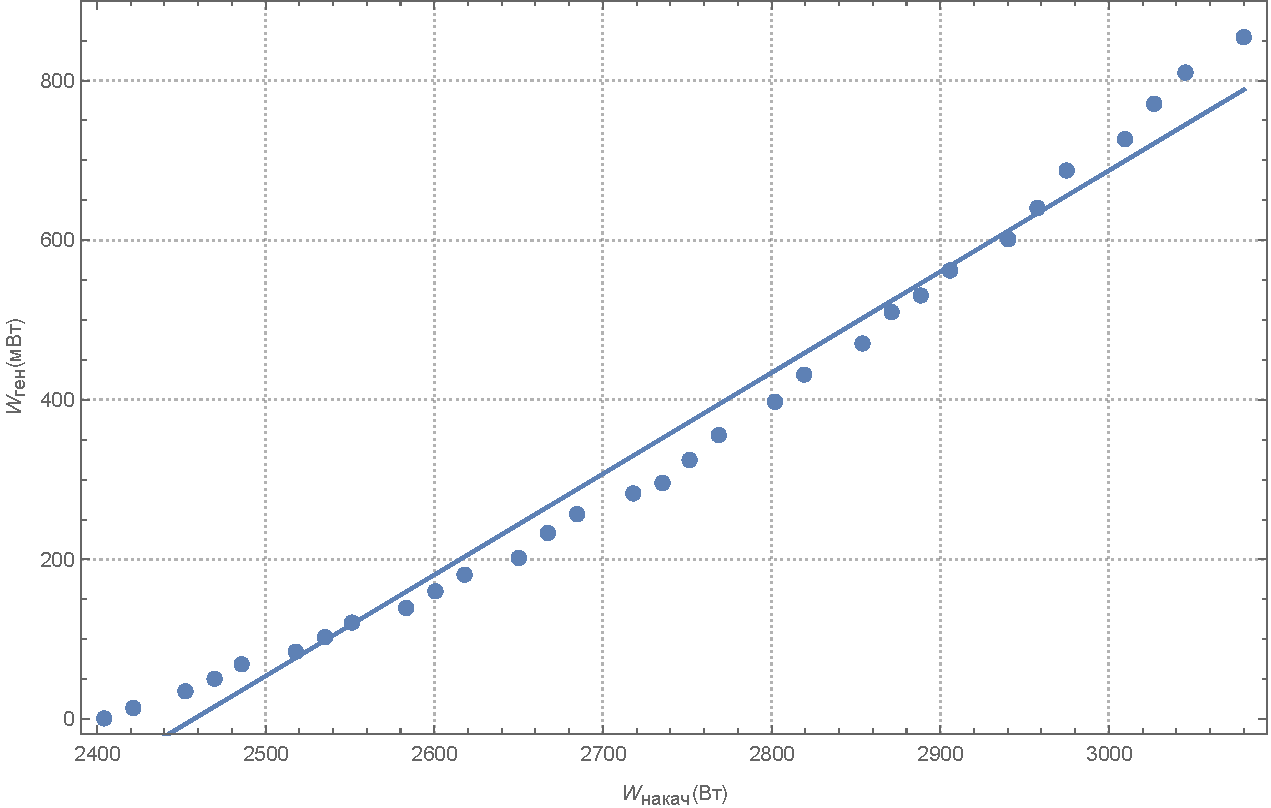
\includegraphics[width=\textwidth]{2.pdf}
	\caption{Зависимость мощности излучения от мощности накачки в режиме модуляции добротности}
	\endminipage
\end{figure}
\begin{table}[!htb]
	\centering
	\caption{Результаты измерения зависимости длительности импульса от мощности накачки лазера в режиме модуляции добротности.}
	\begin{tabular}{|c|c|c|c|}
		\hline
		$I$, А & $U$, В & $t$, мкс & $W$, Вт\\
		\hline
		17.4 & 177. & 0.38 & 3079.8 \\
 17.2 & 176. & 0.33 & 3027.2 \\
 17. & 176. & 0.34 & 2992. \\
 16.8 & 175. & 0.34 & 2940. \\
 16.6 & 175. & 0.38 & 2905. \\
 16.4 & 174. & 0.42 & 2853.6 \\
 16.2 & 173. & 0.34 & 2802.6 \\
 16. & 173. & 0.37 & 2768. \\
 15.8 & 172. & 0.42 & 2717.6 \\
 15.6 & 171. & 0.45 & 2667.6 \\
 15.4 & 170. & 0.54 & 2618. \\
 15.2 & 170. & 0.52 & 2584. \\
 15. & 169. & 0.56 & 2535. \\
 14.8 & 169. & 0.7 & 2501.2 \\
 14.6 & 168. & 0.84 & 2452.8 \\
 \hline
	\end{tabular}
\end{table}
\begin{figure}[!htb]
	\centering
	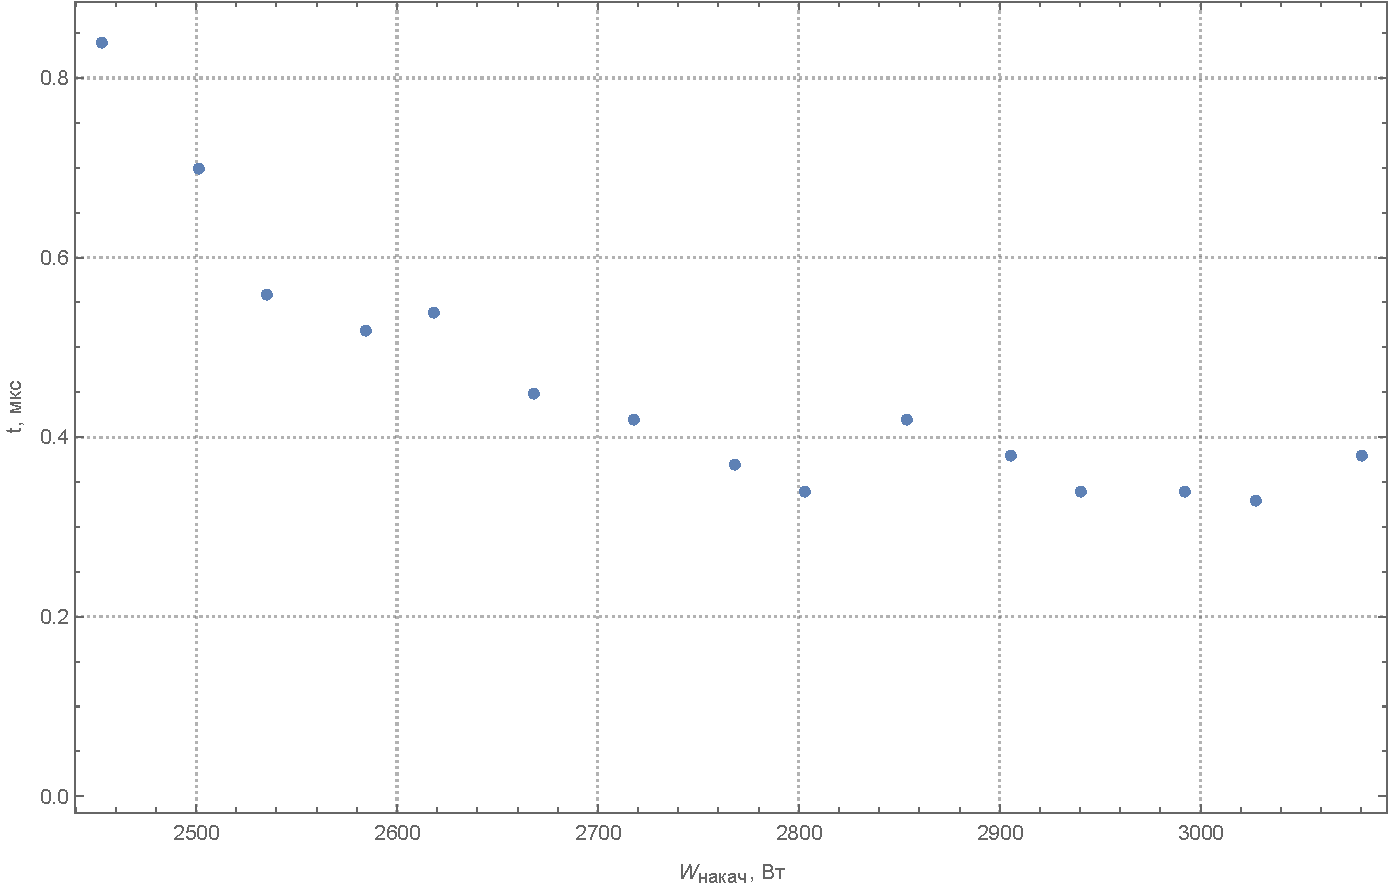
\includegraphics[width=\textwidth]{3.pdf}
	\caption{График зависимости длительности импульса от мощности накачки}
	\label{timeOfPower}
\end{figure}
\section{Анализ полученных результатов}
По графикам определим КПД лазера в разных режимах работы, как угловой коэффициент наклона аппроксимирующей прямой:
$ \eta_{CW} \approx (0,14 \pm 0,02)\% $ и 
$ \eta_{QW} \approx (0,13 \pm 0,02)\% $. Это незначительное различие можно объяснить меньшим средним значением инверсии населённости уровней и, как следствие, меньшими потерями на спонтанное излучение.

Также определим пороговую мощность 
$ W_{CW} \approx (2505 \pm 125) $ Вт и 
$ W_{CW} \approx (2457 \pm 95) $ Вт соответственно. Близость этих значений объясняется равенством потерь в резонаторе в обоих случаях.

На рисунке \ref{timeOfPower} видна логарифмическая зависимость времени импульса от мощности накачки, которая видна и в формуле оценки длительности импульса:
\begin{equation}
	\Delta\tau_p=\tau_c\frac{(N_i/N_p)\eta_E}{\left(\frac{N_i}{N_p}\right)-\ln\left(\frac{N_i}{N_p}\right)-1}=\tau_c\frac{-\ln(1-\eta_E)}{\left(\frac{N_i}{N_p}\right)-\ln\left(\frac{N_i}{N_p}\right)-1}
\end{equation}
На рисунке \ref{impulse} представлено фото изображения импульса на экране осциллографа:
\begin{figure}[h]
	\centering
	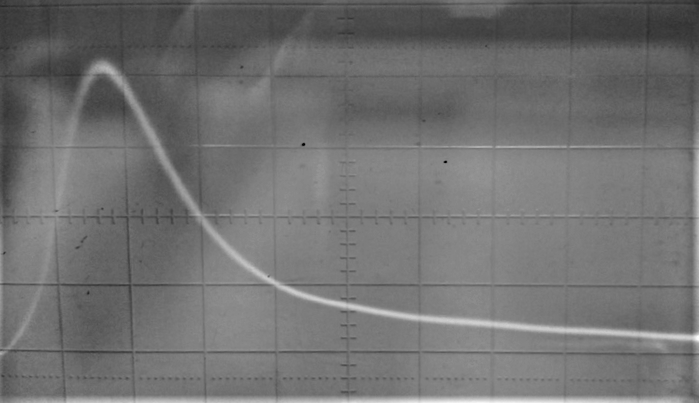
\includegraphics[scale=0.5]{impuls}
	\caption{Внешний вид импульса на экране осциллографа.}
	\label{impulse}
\end{figure}
\section{Гравировка изображения}
Для демонстрации технических возможностей лазера была произведена гравировка изображения.
\begin{figure}[!htb]
	\centering
	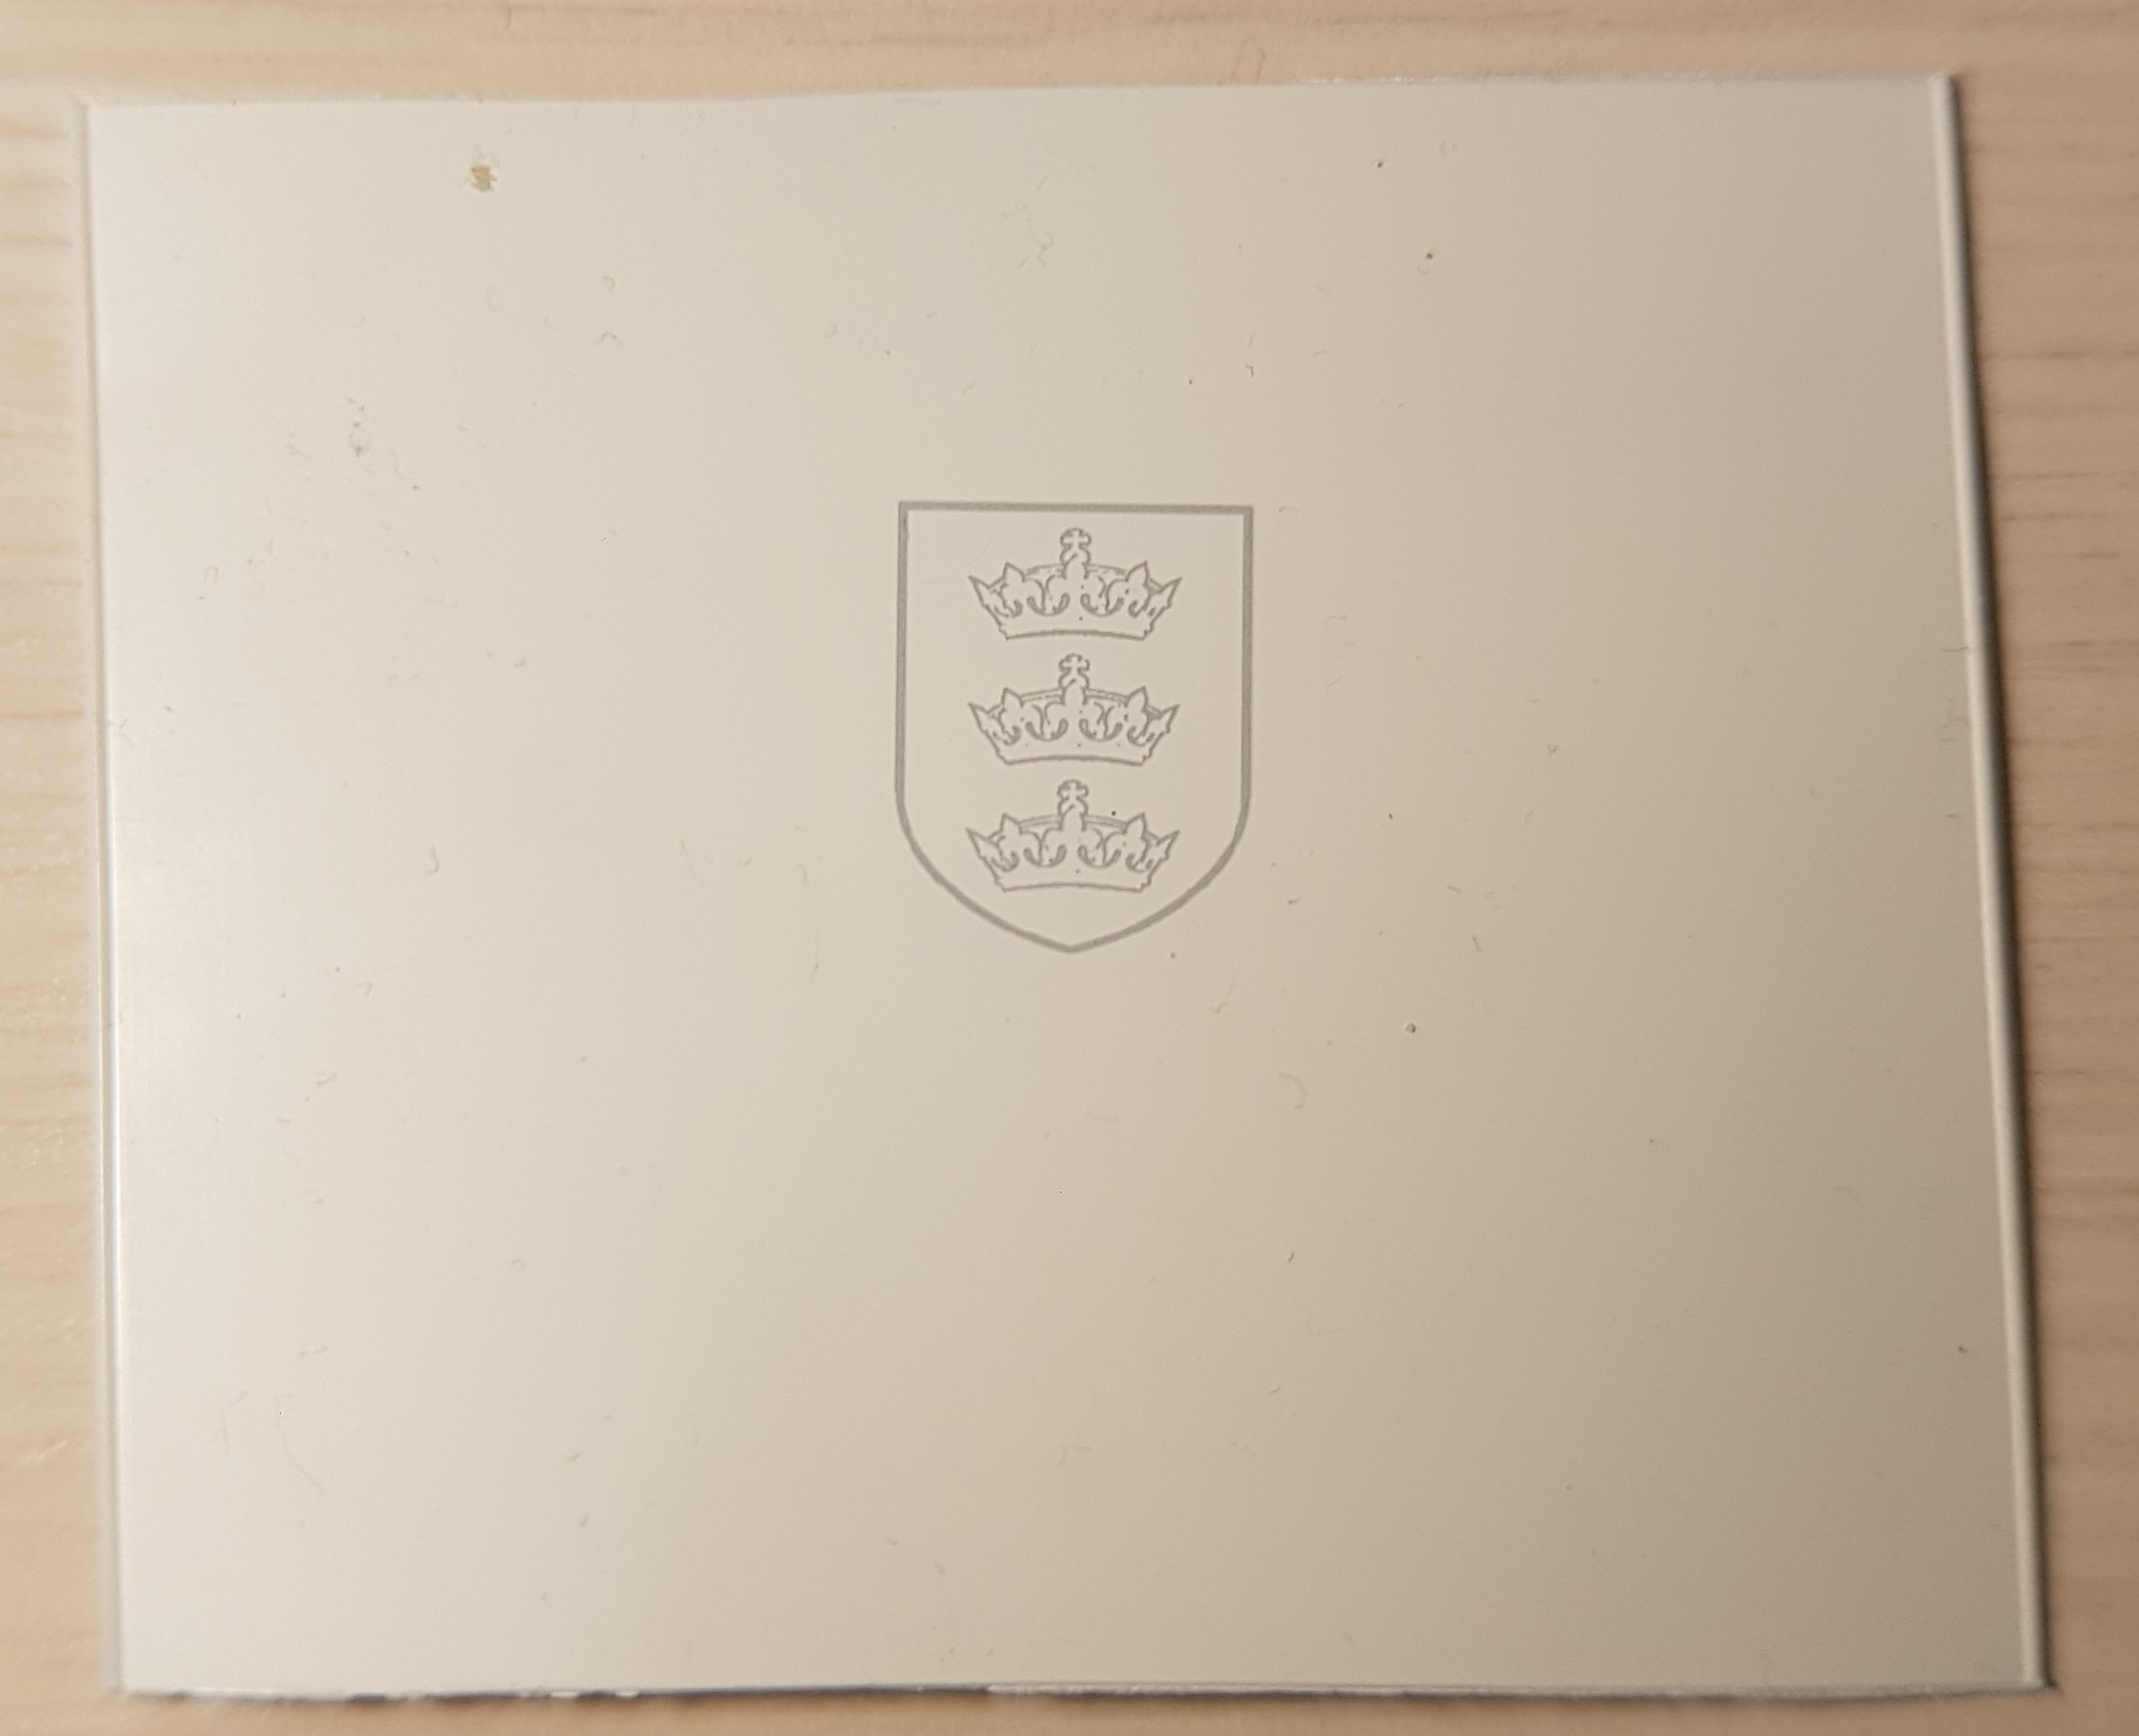
\includegraphics[scale=0.12]{card.jpg}
	\caption{Выгравированное изображение}
\end{figure}
\section{Вывод}
Были изучены физические основы работы различных режимов лазера и определены КПД и пороговая мощность:
\begin{table}[h!]
		\centering
		\begin{tabular}{|c||c|c|}
			\hline
			Режим & Свободной генерации   & Модуляции добротности \\ 					\hline
			$\eta$,~\%   & 0,14 & 0,13 \\ \hline
			$P_{\text{пор}}$, Вт    & 2505 & 2457 \\
			\hline
		\end{tabular}
	\end{table}\par
	В режиме модуляции добротности КПД лазера меньше, чем в непрерывном режиме. Это связано с тем, что в режиме модуляции добротности инверсная населённость в среднем больше (потому что в данном случае отсутствует вынужденное излучение при закрытом модуляторе), чем в непрерывном режиме, а значит, больше потери на спонтанное излучение.\par
	При достижении пороговой мощности усиление в активной среде становится равным потерям в резонаторе, поэтому пороговая мощность не должна зависеть от режима работы. Это и было получено в работе, так как мощности оказались равны в пределах погрешности.
\section{Задачи}
\subsection*{Задача 1}
Считаем для простоты $\eta=100\%$, тогда
\begin{equation*}
	E=N\cdot\tau=mC_{\text{тв}}(T_1-T_0)+mC_{\text{ж}}(T_2-T_1)+m\Lambda+mQ
\end{equation*}
где $m=\rho_{\text{ар}}\cdot V=2.7\cdot10^{-3}$ г, $C_{\text{тв}}$ и $C_{\text{ж}}$ -- удельные теплоемкости Al в твердом и жидком состояниях соотвественно, $\Lambda,\ Q$ -- теплоты плавления и парообразования, $T_0$ -- комнатная температура, $T_1,\ T_2$ -- температуры плавления и кипения (при 1 атм). Таким образом $E\approx 37.34$ Дж. Учтем коэффициент отражения $T=0.93\Rightarrow E\approx 34.73$ Дж.
\subsection*{Задача 2}
Из теории диффракции Фраунгофера
\begin{equation*}
	\psi=\frac{1.22\lambda}{D}\approx 1.3\cdot 10^{-4}\text{ рад}.
\end{equation*}
\subsection*{Задача 3}
\begin{enumerate}
\item Будем считать, что линза расположена в области перетжки пучка. Чтобы найти $d$ пучка в области следующей перетяжки, обратимся к теории Гауссовых пучков и введем комплексный параметр $q$:
\begin{equation*}
	\frac{1}{q}=\frac{1}{R}-\frac{i\lambda}{\pi r^2},
\end{equation*}
где $R(z)$ -- радиус кривизны пучка, $r(z)$ -- поперечный радиус пучка.
\item Если оптическая система описывактся матрицей $A=\left(\begin{matrix}
a & b\\
c & d
\end{matrix}\right)$, то периметр $q_2$ на выходе системы связан с параметром $q$, на входе как
\begin{equation*}
	q_2=\frac{aq_1+b}{cq_1+d}
\end{equation*}
Для системы из собирающей линзы и свободного пространства имеем:
\begin{equation*}
	A(z)=\left(\begin{matrix}
	1-\frac{z}{f} & z\\
	-\frac{1}{f} & 1
	\end{matrix}
	\right)
\end{equation*}
Тогда формула для параметра принимает вид:
\begin{equation*}
	\frac{1}{q(z)}=\frac{1-q(0)/f}{\left(1-\frac{z}{f}\right)q(0)+z}
\end{equation*}
\item Обозначим координату следуюшей перетяжки как $z_m$. Так как в областях перетяжки $R=\infty$, то $q(0)$ и $q(z_m)$ -- чисто мнимые величины:
\begin{equation*}
	q(0)=i\cdot\frac{\pi d_0^2}{4\lambda}=i\cdot z_0,
\end{equation*}
поэтому величину $z_m$ найдем из:
\begin{equation*}
	\text{Re}\frac{1-i\frac{z_0}{f}}{\left(1-\frac{z_m}{f}\right)q(0)+z_m}=0\longrightarrow z_m=\frac{fz_0^2}{f^2+z_0^2}	
\end{equation*}
т.к. $z_0=295$ см $\gg f=20$ см $\Rightarrow$ считаем, что $z_m=f$, т.е. диаметр минимален в фокусе линзы. Тогда
\begin{equation*}
	\text{Im}\frac{1}{q}(z_m)=-\frac{4\lambda}{\pi d^2}\Rightarrow d=\frac{4\lambda f}{\pi d_0}=0.677\ \text{мм}
\end{equation*}
\item В свободном пространстве для функции $r(z)$ (при $r(0)$ -- область перетяжки) имеем:
\begin{equation*}
	r(z)=r(0)\cdot\sqrt{1+\left[\frac{\lambda z}{\pi r(0)^2}\right]^2}
\end{equation*}
тогда условие $r(z)<\sqrt{2}\cdot r(0)$ выполняется внутри области шириной $z_c=2\cdot\frac{\pi r(0)^2}{\lambda}=2z_0=584$ м.
\end{enumerate}
\section*{Задача 4}
Глубина отверстия:
\begin{equation*}
h=\sqrt[3]{\left(\frac{r_0}{\tan\varphi}\right)^3+\frac{3E}{x\tan^2\varphi L_0}}-\frac{r_0}{\tan\varphi}=0.005\text{ м}.
\end{equation*}
Ширина:
\begin{equation*}
	d=2\sqrt{r_0^3+\frac{3E\tan\varphi}{\pi L_0}}=22.8\text{ см}
\end{equation*}
\section*{Задача 5}
Время жизни $\tau_c=\frac{2L'}{\gamma c}$, где $L'=(L-l)+n\cdot l$ -- оптическая длина резонатора, $r=-\ln\left((1-T)^2R_1R_2\right)$ -- потери за проход. $R_2=1-Q_2=80\%$ -- коэффициент пропускания зеркала , $T$ -- относительные внтуренние потери. $T_1=\frac{(L-l}+hl{-\ln((1-T)^2\cdot R_1R_2)}=687.6$ нс.
\section*{Задача 6}
\begin{enumerate}
	\item $P_{\text{изл}}=\frac{h\nu}{2\tau_c}q$, $q$ -- число фотонов в резонаторе.
	\item $q$ в стационарном состоянии находим из скоростных уравнений, приняв $\frac{dN}{dt}=0$ и $\frac{dq}{dt}=0$:
	\begin{equation*}
		\begin{cases}
			R_p=BqN+\frac{N}{\tau}\\
			BV_aN=\frac{1}{\tau_c}
		\end{cases},
	\end{equation*}
где $V_a$ -- объем активного элемента, $B=\frac{\sigma c}{v}$ -- константа Эйнштейна, $V=\frac{L'}{l}V_a$ -- объем резонатора, $\tau$ -- время жизни верхнего уровня.

$q=V_a T_c R_p-\frac{1}{B\tau}=\frac{h}{B\tau}\left(\frac{P_{\text{нак}}}{P_{\text{порог}}}-1\right)\Rightarrow P_{\text{изл}}=\frac{h\nu}{2 T_c}\frac{1}{B\tau}\left(\frac{P_{\text{нак}}}{P_{\text{порог}}}-1\right)=21$ Вт.\\
$P_{\text{порог}}=\frac{1}{\frac{B\tau\eta}{Slh\nu}}=2.5$ кВт.
\end{enumerate}
\section*{Задача 7}
\begin{enumerate}
\item При закрытом модуляторе скоростное уравнение
\begin{equation*}
	\frac{dN}{dt}=R_p-\frac{N}{\tau}
\end{equation*}
пологая $N(0)=0\Rightarrow N(t)=R_p\tau(1-e^{-\frac{t}{\tau}})$
\item Сделаем грубую оценку: пусть длительность импульса модуляции равна половине периода $T=\frac{1}{\nu}$, в момент закрытия модулятора модулятора $N=0$, тогда $N_i=R_p\tau(1-e^{\frac{T}{2\tau}})=0.05 R_p\tau$.
\item Для нахождения $R_p=\frac{\nu P_{\text{нак}}}{h\nu V_a}\Rightarrow N_i=6.8\cdot10^{40}$
\end{enumerate}
\section*{Задача 8}
Обозначим $x=\frac{N_i}{N_p}$. Тогда для длительности импульса имеем: $\Delta t=\tau_c\frac{x\eta_E}{x-\ln x-1}$. $N_p=\frac{\gamma}{\sigma l}=8\cdot 10^{22}\ \text{м}^{-3}\Rightarrow x=2.62$. Из графика зависимости $\eta_E\left(\frac{\text{эффективная населенность}}{\min\text{ населенность}}\right)$ находим $\eta_E=0.9\Rightarrow\Delta t=50$ нс.
\section*{Задача 9}
$E=\left(\frac{-\ln(R_2)c}{2Le}\right)(h\nu_p)\cdot\int_0^\tau\Phi dt=\left(\frac{\ln(R_2)}{2\ln((10L)\sqrt{R_1R_2}}\right)(N_i-N_f)(V_ahV_l)$, где $N_i\approx 0.05\eta\frac{P_{\text{нак}}}{slh\nu}\tau\approx E\sim P_{\text{нак}}$.
\section*{Задача 10}
$x=\frac{N_i}{N_p}\uparrow\uparrow\Rightarrow E\uparrow\uparrow$. $N_p$ не зависит от частоты. Чем меньше частота, тем больше времени происходит накачка фотонов $\Rightarrow N_o\uparrow\uparrow\Rightarrow x\uparrow\uparrow\Rightarrow$ с ростом частоты модулятора $E$ в импульсе $\downarrow\downarrow$, и наоборот.
\section*{Задача 11}
Из задачи 9: $E\sim 10^{-4}$ Дж.
\end{document}